
\section{Metrics on the shape space}
\label{sec:metrics-shape-space}
In the previous sections we defined and deduced some properties of our shape space of interest. We also defined a metric induced by the $L^2$-inner product. In this section we consider this metric and another in more depth.

\subsection{The L2 metric vanishes}
\label{sec:l2-metric-vanishes}

In the previous section we went through some work to construct a measure of length for a path $q$ in the space $\mathcal{I}$. As the tangent spaces were seen to consist of some functions on the circle, it was natural to consider using a version of the L$^2$-metric (a version invariant to reparametrizations). However, as we illustrate in this section, this does not give rise to a usable notation of length, because the geodesic distance following from this metric becomes 0 for every two curves in the space.

It can seem weird to go through so much trouble to define a useless distance. But firstly, the construction illustrates some of the difficulties in defining a reasonable notion on length on $\mathcal{I}$; secondly, and more importantly, the fact that the distance vanishes is a quite surprising result, which depends crucially on the formula for the length of a path given in Proposition~\ref{prop:length-quotient}. This gives us some justification for the somewhat unfruitful work of defining the L$^2$-metric.

The ``proof'' below is mostly heuristic, and we only consider the very simple case of a path transforming the circle into a larger circle, but this captures the main idea.
\begin{theorem}
  \label{theorem:l2-metric-vanishes}
  For all $\mathrm{a},\mathrm{b} \in \mathcal{I}$
  \begin{equation*}
    \mathcal{D}(\mathrm{a},\mathrm{b}) = 0.
  \end{equation*}
\end{theorem}

\begin{proof}[Proof of Theorem~\ref{theorem:l2-metric-vanishes}]

  \begin{figure}
    \centerline{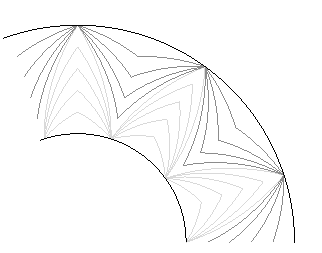
\includegraphics[width=0.6\linewidth]{zigzag-path0.pdf}}
    \caption[]{Illustration of a zigzag path moving the unit circle to the circle with radius 2. The path first moves the points along the path sketched in light-grey and then moves them along the dark-grey path.}
    \label{fig:zigzag-path}
  \end{figure}

  By the definition of the length $\mathcal{D}$ we need to show that for any two paths $\mathrm{a},\mathrm{b} \in \mathcal{I}$ and any $\epsilon >0 $ there exists a path $\mathrm{q}$ in $\mathcal{I}$ such that
  \begin{equation*}
    \mathcal{L}(\mathrm{q}) < \epsilon.
  \end{equation*}
  The trick is to construct a path in $\I$ that moves in zigzag and then use Proposition~\ref{prop:length-quotient} to calculate the length of this path in $\mathcal{I}$.
  It turns out that when we increase the number of teeth of the zigzag path, the length of the path decreases in $\mathcal{I}$.
  The idea of such a zigzag path is illustrated in figure~\ref{fig:zigzag-path}.

  To see why this  phenomenon happens, first rewrite \eqref{eq:length-quotient} from Proposition~\ref{prop:length-quotient} as
  \begin{align*}
    \mathcal{L}(q) &
                     = \int_{0}^{1}
                     \left(
                     \int_{\S^{1}} \frac{\langle q_{t},i q_{\theta}\rangle^2}
                     {|q_{\theta}|}  \diff \theta
                     \right)^{1/2} \diff t \\
                   & =  \int_{0}^{1}
                     \left(
                     \int_{\S^{1}}
                     \left(
                     \frac{\langle q_{t},i
                     q_{\theta}\rangle}{| q_{t}|| q_{\theta}|}
                     \right)^2
                     | q_t|^2   | q_{\theta}|
                     \diff \theta
                     \right)^{1/2} \diff t \\
                   &  =
                     \int_{0}^{1}
                     \left(
                     \int_{\S^{1}}
                     \cos(\alpha( q_t, i q_{\theta}))^2
                     | q_t|^2   | q_{\theta}|
                     \diff \theta
                     \right)^{1/2}\diff t,
  \end{align*}
  with $\alpha(x,y)$ denoting the angle between $x$ and $y$.
  When constructing a zigzag-path the angle will for large enough $n$ be given approximately by
  \begin{equation}
    \label{eq:tan-angle}
    2n \approx \tan(\alpha).
  \end{equation}
  Note that this does not depend on $\theta$ nor $t$.
  See figure~\ref{fig:angle-arg} for a visual justification of this.
  \begin{figure}[h]
    \centering
    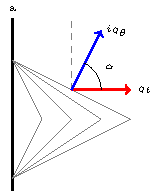
\includegraphics[width=0.5\linewidth]{angle-argument.pdf}
    \caption{Relative to $q_t$, $iq_{\theta}$ is by construction a line with slope $2n$, and thus the angle between these two vectors are found by \eqref{eq:tan-angle}. Note that the starting curve, $\mathrm{a}$, is here represented as a straight line to simplify the calculations; this should be a reasonable approximation when $n$ is large.}
    \label{fig:angle-arg}
  \end{figure}

  We have that
  \begin{equation*}
    \cos(\arctan(2n)) = (1+(2n)^2)^{-1/2}
    = O(n^{-1}),
  \end{equation*}
  so we can write
  \begin{equation}
    \label{eq:approx-L-angle}
    \begin{aligned}
    \mathcal{L}( \mathrm{q} )
    & =
      \int_{0}^{1}
      \left(
      \int_{\S^{1}}
      O(n^{-1})^2
      | q _t|^2   | q _{\theta}|
      \diff \theta
      \right)^{1/2} \diff t \\
    & =
      O(n^{-1})
      \int_{0}^{1}
      \left(
      \int_{\S^{1}}
      | q _t|^2   | q _{\theta}|
      \diff \theta
      \right)^{1/2} \diff t.
    \end{aligned}
  \end{equation}
  To show that our zigzag path has arbitrary small length we thus just need to show that the remaining integral does not grow faster than $n$. Figure~\ref{fig:zigzag-path-angle} illustrates how the angle $\alpha$ increases towards $\pi/2$, making $\cos(\alpha) \rightarrow 0$; at the same time, it is seen how $q_{\theta}$ grows -- not fast enough, however, to kill the $\cos(\alpha)$ term, it turns out.

\begin{figure}
  \centering
  \begin{subfigure}{.49\textwidth}
    \centering
    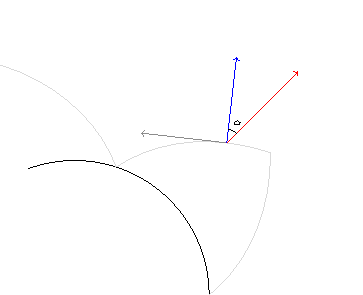
\includegraphics[width=1\linewidth]{zigzag-path.pdf}
  \end{subfigure}
  \begin{subfigure}{.49\textwidth}
    \centering
    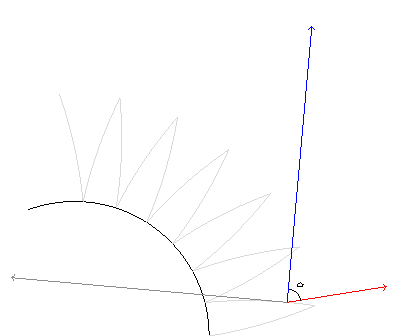
\includegraphics[width=1\linewidth]{zigzag-path2.pdf}
  \end{subfigure}
  \caption{Illustration of how the angle $\alpha$ increases with the number of teeth of the zigzag path. The red vector gives the time derivative, the grey the path derivative, and the blue the normal of the path derivative. The zigzag path is shown in light-grey in the background. (Note that the length of the vectors are scaled to fit the drawing and does not necessarily reflect an exact relationship between the lengths of the two.)}
  \label{fig:zigzag-path-angle}
\end{figure}

As an example, we take the simple case where we expand the circle $e^{i\pi\theta}$ to
$2e^{i\pi\theta}$. The zigzag path is then concretely given as
\begin{equation*}
  \phi(t,\theta) = e^{i\pi\theta}
  \sum_{k=0}^{n-1}
  h^{n,k}(t,\theta) + g^{n,k}(t,\theta)
\end{equation*}
where
\begin{equation*}
  \begin{aligned}
    h^{n,k}(t,\theta) & := 1_{[\frac{k}{n},\frac{k}{n} +
      \frac{1}{2n})}(\theta) \left( 1+2t(n\theta-k) \right), \\
    g^{n,k}(t,\theta) & := 1_{[\frac{k}{n} + \frac{1}{2n},\frac{k+1}{n})}(\theta)
    \left( 1+2t(1-n\theta-k) \right).
  \end{aligned}
\end{equation*}
We have that
\begin{equation*}
  \begin{aligned}
    |\phi_t| & = \sum_{k=0}^{n-1} |h^{n,k}_t| + \sum_{k=0}^{n-1}
    |g^{n,k}_t|, \\
    |\phi_{\theta}| & = \sum_{k=0}^{n-1} |h^{n,k}_{\theta} + h^{n,k} | +
    \sum_{k=0}^{n-1}
    |g^{n,k}_{\theta} + g^{n,k} |,
  \end{aligned}
\end{equation*}
so by symmetry
\begin{equation*}
  \begin{aligned}
    \int_{0}^{1}
    |\phi_t|^2   |\phi_{\theta}|
    \diff \theta
    & =
    2n \int_{0}^{\frac{1}{2n}} |h^{n,0}_t|^2 |h^{n,0}_{\theta} + h^{n,0} |
    \diff \theta \\
    & = 2n \int_{0}^{\frac{1}{2n}}
    (2n\theta)^2(2tn+1+t2n\theta) \diff \theta \\
    & = \int_{0}^1
    u^2(2tn+1+t u) \diff \theta \\
    & = O(n),
  \end{aligned}
\end{equation*}
for $t\in[0,1]$. Plugging this into \eqref{eq:approx-L-angle} gives the result.
\end{proof}

The above result shows that the simple $L^2$-metric is unfortunately not a fruitful way for imposing a metric structure on our shape space. To do this, more complicated metrics that take more of the functions properties into account is needed. One fairly straightforward generalisation of the $L^2$ metric are Sobolev metrics that take some of the derivatives of a function into account. Another approach is to consider so-called \textit{almost local metric}, which we do in the following section.


%%% Local Variables:
%%% mode: latex
%%% TeX-master: "mainfile"
%%% End:
